\lecture{13}{Sun 13 Nov 2022 18:04}{Series Representation}


\section{Series Representation}
\subsection{Series}

In real calculus, if $f$ is infinitely differentiable, it is not true that it can be written as a convergent taylor series. $f^{(n)}(a)$ may have all derivatives, but Taylor series diverge, or conerge to another function.
\begin{example}
	Define $f(x) = \begin{cases}
		0 & x\le 0\\
		e^{- \frac{1}{x}} & x>0
	\end{cases}$
	. This function is continuous and infinitely differentiable. But all derivatives at $0$ is $0$, so the taylor series is $0$.
\end{example}

However, in complex analysis, all holomorphic functions are analytic, i.e. all difinitely differentiable functions have taylor series representation.

\begin{definition}[Series]
	Let $S_n = a_0 + \ldots+ a_n$ be the n-th partial sum. If $\lim_{n \to \infty} S_n = s$ exists, call $s$ the sum of the series.

	The series is called \textit{convergent} if the limit exists.
\end{definition}

\begin{lemma}[Geometric Series]
	Consider the series $1 + q + q^2 + \ldots = \sum_{n=1}^{\infty} q^n$. Multiply by $q$ to each term, we see that $1 + qS_n = S_n + q^{n+1}$. We see that $s_n = \frac{1 - q^{n+1}}{1 - q}$.

	If $|q| < 1$ then
	\[
		\sum_{n=1}^{\infty} q^n = \frac{1}{1-q}
	.\]
	 If $|q| \ge 1$ then the limit does not exist.
\end{lemma}

\begin{definition}[Absolutely Convergent]
	A series is called \textit{absolutely convergent} if $\sum_{n=1}^{\infty} |a_n|$ is convergent.
\end{definition}

\begin{example}
	Consider the series $\sum_{n=1}^{\infty} n^{- \alpha}$, $\alpha \in \mathbb{R}$.

The sum is bounded above by $\int_1^{\infty } \frac{dx }{x^\alpha}= - \frac{1}{1-\alpha}$, but this is reasonable when $\alpha > 1$. So the series is convergent when $\alpha>1$.

When $\alpha = 1$, we can have a lower estimate by integral, and the integral is divergent. Hence the harmonic series diverges.
\end{example}

\begin{example}
	 \[
		1 - \frac{1}{2} + \frac{1}{3} - \frac{1}{4} + \ldots = \ln 2
	.\] 
	This series is convergent but not absolutely.

	For series that are convergent but not absolutely, we can rearrange to obtain any sum.
\end{example}

Now we give some criterions for convergence.
\begin{theorem}[Comparison Test]
	If the series $\sum_{j=1}^{\infty} c_j$ satisfies that $|c_j| \le  M_j$ for all sufficiently large $j$, and $\sum_{j=1}^{\infty} M_j$ converges (as series of real numbers), then the series $\sum_{j=1}^{\infty} c_j$converges.
\end{theorem}

\begin{theorem}[Ratio Test]
	If the series $\sum_{j=1}^{\infty} c_j$ satisfies that $|\frac{c_{j+1}}{c_j}|  \to L$ as $j \to \infty $, then the series converges if $L < 1$ and diverges if $L > 1$.
\end{theorem}

\subsection{Taylor Series}
\begin{definition}[Taylor Series]
	If $f$ is analytic at $z_0$, then the series
	\[
		\sum_{j=0}^{\infty} \frac{f^{(j)}(z_0)}{j!}(z-z_0)^j
	.\] 
	is called the \textit{Taylor series} for $f$ at $z_0$. When $z_0 = 0$, this is called \logseq{Maclaurin Series}.
\end{definition}

\begin{theorem}[Taylor's Theorem]
	If $f$ analytic in the disk $|z - z_0| < R$, then the Taylor series converges to $f(z)$ for all $z$ in the disk. Also, the convergence is uniform in any closed subdisk $|z - z_0| \le R' < R$.
\end{theorem}
\begin{proof}
	We only prove the argument for uniform convergence in closed subdisk, as it will imply pointwise convergence in whole disk.

	Fix $R'$ and let $C$ be the circle $|z - z_0| = \frac{R + R'}{2}$, positively oriented. By Cauchy's Integral Formula, for every  $z$ within the closed subdisk,
	\[
		f(z) = \frac{1}{2 \pi i} \int_C \frac{f(\xi)}{\xi - z} d \xi
	.\] 
	We use geometric series to rewirte $\xi - z$ as
	\begin{align*}
		\frac{1}{\xi - z} &= \frac{1}{\xi - z_0} \frac{1}{1- \frac{z - z_0}{\xi - z_0}}\\
		&= \frac{1}{\xi - z_0}\left[ 1 + a + \ldots + a^n + \frac{a^{n+1}}{1-a} \right]
	\end{align*} 
	where $a = \frac{z-z_0}{\xi - z_0}$.

	Plug the $k$-th term to the cauchy integral formula, we see
	\[
		\frac{1}{2 \pi i} \int _C f(\xi) \frac{1}{\xi - z_0} a^k d \xi = \frac{(z - z_0)^k}{2 \pi i} \int_C \frac{f(\xi)}{(\xi - z_0)^{k+1}}d \xi
	.\] 
	Using Cauchy Differentiation Formula,
\[
		\frac{(z - z_0)^k}{2 \pi i} \int_C \frac{f(\xi)}{(\xi - z_0)^{k+1}}d \xi = \frac{f^{(k)}(z_0)}{k!}(z-z_0)^k
	.\]
	which is exactly the $k$-th term in Taylor series. Now we only need to show that the remainder term converges to $0$ uniformly. The remainder term is
	\[
		T_n(z) = \frac{1}{2 \pi i}\int _C f(\xi)  \frac{1}{\xi - z_0}\frac{a^{n+1}}{1-a} d \xi = \frac{1}{2 \pi i} \int _C \frac{f(\xi)}{\xi - z} \frac{(z-z_0)^{n + 1}}{(\xi - z_0)^{n+1}} d \xi
	.\] 
	Now apply main estimate. Using the following identities:
	\[
		|z - z_0| < R', \quad |\xi - z_0| < \frac{R + R'}{2}, \quad \frac{|z - z_0|}{|\xi - z_0|}\le \frac{2R'}{R + R'}
	.\] 
	and
	\[
		|\xi - z| \ge \frac{R + R'}{2} - R' = \frac{R - R'}{2}
	.\] 
	We have
	\begin{align*}
		|T_n(z)| &\le \frac{1}{2 \pi} |C| \max_{\xi \text{ on }C} \frac{f(\xi)}{\xi - z} \frac{(z-z_0)^{n + 1}}{(\xi - z_0)^{n+1}}\\
			 &\le \frac{1}{2 \pi} \left( 2 \pi \frac{R + R'}{2} \right) 
\max_{\xi \text{ on }C} |f(\xi)| \frac{2}{R - R'} \left( \frac{2 R'}{R + R'} \right) ^{n+1}
	.\end{align*} 
	Now the term right hnd term does not depend on $z$ and can be made arbitrarily small by increasing $n$.
\end{proof}
	
\begin{remark}
	The taylor series will converge in the \textbf{biggest open disk} around $z_0$ where $f$ is analytic.
\end{remark}

\subsection{Operations on Taylor Series}

\begin{theorem}
	For $f,g$ with convergent taylor series around $z_0$, say $f(z) = \sum_{j=0}^{\infty} a_j (z-z_0)^j$ and $g(z) = \sum_{j=0}^{\infty} b_j (z-z_0)^j$ the followings hold: (we consider taylor series at $z_0$ )
	\begin{itemize}
		\item The taylor series of $f'$ is the term-wise differentiation of taylor series of $f$.
		\item For constant $c$, taylor series of $cf$ is $\sum_{j=0}^{\infty} ca_j(z-z_0)^j$
		\item The taylor series of $f \pm g$ is $\sum_{j=0}^{\infty} (a_j \pm b_j) (z-z_0)^j$ 
		\item The taylor series of $fg$ is the \textit{Cauchy product} of taylor series of $f$ and taylor series of $g$.
	\end{itemize}
\end{theorem}

\begin{definition}[Cauchy Product]
	The \textit{Cauchy product} of two Taylor series $\sum_{j=0}^{\infty} a_j (z-z_0)^j$ and $\sum_{j=0}^{\infty} b_j (z-z_0)^j$ is defined to be the series $\sum_{j=0}^{\infty } c_j(z-z_0)^j$ where
	\[
		c_j = \sum_{l=0}^{j} a_{j-l}b_l
	.\] 
\end{definition}
\begin{intuition}
	We are looking through each term of the two series and summing all ways that a particular power $j$ can be obtained by multiplying together terms from the two series.
\end{intuition}

\subsection{Power Series}

\begin{definition}[Power Series]
	A series of the form $\sum_{j=0}^{\infty } a_j(z - z_0)^j$ is called a  \textit{power series}. The constants  $a_j$ called the \textit{coefficients} of the power series.
\end{definition}

\begin{fact}
	(to establish in the lecture)
	A power series about $z_0$ converges everywhere within its radius of convergence. A convergent power series converges to a function $f$ analytic within its radius of convergence, and the power series is exactly the Taylor series of $f$ at $z_0$.

\end{fact}

The next theorem is not proved in this class. Optional reading.
\begin{theorem}[Radius of Convergence]
	For any power series $\sum_{j=0}^{\infty } a_j(z - z_0)^j$ there is a real number $R$ between $0$ and $\infty $ (inclusive), which independent of $z$, such that
	\begin{enumerate}
		\item The series converges within $|z - z_0| < R$
		\item The series converges uniformly within any closed subdisk.
		\item The series diverges for $|z - z_0| > R$.
	\end{enumerate}
	The real number $R$ is called the  \textit{radius of convergence}.
\end{theorem}
\begin{remark}
	The power series \textbf{must fail to converge somewhere} on circle of convergence, otherwise it must be convergent in a bigger region.
\end{remark}

\begin{theorem}
	Uniform limit preserves continuity of function. If $f_n$ continuous on $T \subset \mathbb{C}$, $f_n \to f$ uniformly on $T$, then $f$ continuous on $T$.
\end{theorem}
\begin{proof}
	omit.
\end{proof}

\begin{theorem}
	\textbf{Uniform limit and integration are exchangeable}. Let $f_n$ be continuous on $T \subset \mathbb{C}$, and  $f_n \to f$ uniformly on $T$. Then for any contour $\Gamma \subset T$, 
	\[
		\int _\Gamma f_n(z) dz \to \int _\Gamma f(z) dz
	.\] 
\end{theorem}
\begin{proof}
	Apply main estimaton.
	\begin{align*}
		&\left|\int _\Gamma f_n(z) dz - \int _\Gamma f(z) dz\right|\\
		&= \left| \int _\Gamma (f(z) - f_n(z)) dz\right|   \\
		&\le \varepsilon |\Gamma|
	.\end{align*}
	Where $\varepsilon > 0$ can be made arbitrarily small, by uniform convergence of $f_n$ to $f$. $|\Gamma|$ is fixed, so we are done.
\end{proof}


\begin{theorem}
	In a simply connected region, uniform limit preserves analyticity of function. If $f_n$ are analytic in a simply connected domain $\mathcal{D}$ and converge uniformly to $f$ in $\mathcal{D}$, then $f$ analytic in $\mathcal{D}$.
\end{theorem}
\begin{proof}
	$f$ continuous since $f_n$ are continuous and the convergence is uniform. Then 
	\[
		\int_\Gamma f dz = \int _\Gamma \lim_{n \to \infty} f_n dz = \lim_{n \to \infty} \int _C f_n dz = 0
	.\] 
	Where the integration over each $f_n$ is zero, since $f_n$ analytic and $\mathcal{D}$ simply connected.
	Hence $f$ analytic by Morera's Theorem.
\end{proof}

\begin{theorem}
	If $\sum_{j=0}^{\infty} a_j (z-z_0)^j$ converges to $f(z)$ in some circular neighborhood of $z_0$, then $f(z)$ is analytic, and the series is exactly the Taylor expansion of $f$ at $z_0$.
\end{theorem}
\begin{proof}
	Any point within the circle of convergence is contained in some closed subdisk, where the convergence of series is uniform. Hence the last theorem applies and $f$ is analytic within the circle of convergence.

	Now pick any positively oriented circle centered at $z_0$ lying inside circle of convergence. Apply Cauchy differentiation formula,
	\[
		f^{(n)}(z_0)=\frac{n !}{2 \pi i} \int_{\partial \mathcal{D}} \frac{f(\zeta)}{(\zeta-z_0)^{n+1}} d \zeta
	\]
	Plug in the power series for $f$ and integrate term-wise:
	\[
		f^{(n)}(z_0)=\frac{n !}{2 \pi i} \sum_{j=0}^{\infty } a_j \int_{\partial \mathcal{D}} \frac{(\zeta-z_0)^j}{(\zeta-z_0)^{n+1}} d \zeta
	.\] 
	Now the integral is $0$ whenever $j\neq n$, and the integral equals to $2 \pi i$ when $j = n$. Hence
	\[
		f^{(n)}(z_0) = a_n n!
	.\] 
	Substitute $a_n$ to the power series and we obtain its taylor series.
\end{proof}

\subsubsection{Computation Examples}
Several Techniques to compute series representation:
\begin{enumerate}
	\item (Geometric Progression; Termwise Differentiation)
		\begin{example}
			Expand $\frac{1}{\left( z-1 \right)^3 }$ at $0$.

			\begin{align*}
				\frac{1}{\left( z-1  \right) ^3}
				&= \frac{1}{2} \frac{d^2}{dz^2}\left( \frac{1}{1-z} \right)  \\
				&= \frac{1}{2}\frac{d^2}{dz^2}\sum_{j=0}^{\infty} z^j \\
				&= \sum_{j=0}^{\infty} \frac{1}{2}(j+2)(j+1)z^j
			.\end{align*}
		\end{example}
	\item (Partial Fraction Decomposition)
		\begin{example}
			Expand $\frac{1}{z^2 + 1}$ at $z=1$.

			Decompose:
			\[
				\frac{1}{z^2 + 1} = \frac{1}{2 i}\left( \frac{1}{z-i} - \frac{1}{z+i} \right) 
			.\] 
			Decompose each independently:
			\begin{align*}
				\frac{1}{z-i} &= \frac{1}{(z-1) - (i-1)} \\
				&= \frac{1}{1-i} \frac{1}{1- \frac{z-1}{i-1}} \\
				&= \frac{1}{1-i} \sum_{j=0}^{\infty} (i-1)^{-j}(z-1)^j \\
				&= - \sum_{j=0}^{\infty} (i-1)^{-j-1} (z-1)^j 
			.\end{align*}
			\begin{align*}
				\frac{1}{z+i} &= \frac{1}{(z-1) - (-i-1)}\\
				&= \frac{1}{i+1} \frac{1}{1 - \frac{z-1}{-i-1}} \\
				&= \sum_{n=1}^{\infty} (-1)^n (i+1)^{-n-1} (z-1)^n
			.\end{align*}
			Now we sum the two series together.
			\[
				\frac{1}{z^2 + 1} = \sum_{n=0}^{\infty} c_n (z-1)^n
			.\] 
			where 
			\[
				c_n = \frac{1}{2} (-1)^n \left( (i+1)^{n-1} + (1-i)^{-n-1}\right) 
			.\] 
		\end{example}
	\item (Taylor Series)
		\begin{example}
			Find power series of the principal branch of $f(z) = (1+z)^{\alpha}$.

			\begin{gather*}
				f(0) = 1 \\
				f'(0) = \alpha(1+a)^{\alpha-1 }|_{z = 0} = \alpha\\
				f^{(n)}(0) = \alpha (\alpha-1) \ldots (\alpha - n + 1)
			\end{gather*}
			Hence
			\[
				f(z) = 1 + \sum_{n=0}^{\infty} \frac{\alpha (\alpha-1) \ldots (\alpha - n + 1)}{n!}z^n
			.\] 
			This is the \logseq{Newton's Binomial Theorem}.

			When $\alpha = m$ is integer,
			\[
				f(z) = \sum_{n=0}^{m} \binom{m}{n} z^n
			.\] 

			When $\alpha = \frac{1}{2}$,
			\[
				\sqrt{1+z}  = 1 + \frac{1}{2} z - \frac{1}{8}z^2 + \frac{3}{24} z^3 - \ldots
			.\] 
		\end{example}
		\begin{example}
			Expand $f(z) = \operatorname{Log} (1+z)$ at $0$, $R = 1$.

			Find derivatives iteratively:
			\begin{gather*}
				f(0) = 0\\
				f'(0) = \frac{1}{1+z} \big|_0 = 1\\
				f''(0) = - \frac{1}{(1+z)^2}\big|_0 = -1
			\end{gather*}
			So
			\[
				f^{(n)}(0) = (-1)^{n-1} (n-1)!
			.\] 
		\end{example}
	\item (Dividing Series)
		\begin{example}
			Expand $f(z) = \tan(z)$ at $0$. $f$ is analytic where $\cos z \neq 0$, where $z \neq  \frac{\pi}{2} + \pi k$. So $R = \frac{\pi}{2}$.

			We express  $\tan(z)$ as ratio os $\sin$ and $\cos$, and expand separately, and then divide them.

			\begin{align*}
				\tan(z) &=  \frac{\sin(z)}{\cos(z)} \\
				&= \frac{z - \frac{z^3}{6 }+ \frac{z^5}{120}+ \ldots}{1 - z^2 + \frac{z^4}{24}- \ldots} \\
				&= \frac{z - \frac{z^3}{6 }+ \frac{z^5}{120}+ \ldots}{1 - (z^2 - \frac{z^4}{24}+ \ldots)} \\
				&=  \left( z - \frac{z^3}{6 }+ \frac{z^5}{120}+ \ldots \right)\left( 1 + \left( z^2 - \frac{z^4}{24}+ \ldots \right) + \left( z^2 - \frac{z^4}{24}+ \ldots \right)^2 + \ldots \right)
			.\end{align*}
			From now on we calculate the Cauchy product of these series. This is doable by hand if only the first few terms are needed.
		\end{example}
\end{enumerate}

\subsubsection{Solving Differential Equations}

\begin{enumerate}
	\item (Compute the derivatives)
\begin{example}[Exponential Function]
	Define the system of ODE
	\[
		\begin{cases}
			y' = y \\
			y(0) = 1
		\end{cases}
	.\] 
	Then by induction $y^{(n)}(0) = 1$ for all $n\ge 0$. Hence by Taylor's Formula,
	\[
		y(z) = \sum_{n=0}^{\infty} \frac{z^n}{n!} =: \exp(z)
	.\] 
\end{example}
	\item (Plug power series to the DE)
		\begin{example}
			Solve $y'' = zy, y(0) = 0$.

			We let $y(z) = \sum_{n=0}^{\infty} a_n z^n$.
			Now 
			\begin{gather}
				y' = \sum_{n=1}^{\infty} n a_n z^{n-1} = \sum_{n=0}^{\infty} (n+1) a_{n+1}a^n\\
				y'' = \sum_{n=1}^{\infty} (n+1)n a_{n+1} z^{n-1} = \sum_{n=0}^{\infty} (n+2)(n+1)a_{n+2} z^n
			\end{gather}
			.
			Now plug to the equation:
			\[
				zy = \sum_{n=0}^{\infty} a_n z^{n+1} = \sum_{n=0}^{\infty} (n+2)(n+1)a_{n+2} z^n			.\] 
		The solution is
		\[
			\begin{cases}
				(n+2)(n+1)a_{n+2} = a_{n-1} & n\ge 1\\
				a_2 = 0

			\end{cases}
		.\] 
		Now we have a recurrence formula of step $3$. We may choose $a_0$, $a_1$ arbitrarily.

	\end{example}
	\begin{example}
		Solve the \textit{delayed differential equation} $f'(z) = f(kz)$.

		Use the same method as above, assuming $f(z) = \sum_{n=0}^{\infty} a_n z^n$, we have
		\[
			(n+1)a_{n+1} = k^n a_n
		.\] 
		Thus
		\[
			f(z) = \sum_{n=0}^{\infty} \frac{k^{\frac{n(n-1)}{2}}z^n}{n!}
		.\] 
		$f$ is entire if $|k|<1$, and $f$ is divergent if $|k| > 1$.
	\end{example}
	\begin{example}(Euler)
		Solve $z^2 y' = y - z$.

		We have
		\[
			z^2 \sum_{n=0}^{\infty} (n+1)a_{n+1}z^n = a_0 + (a_1-1)z + \sum_{n=2}^{\infty} a_n z^n
		.\] 
		thus
\[
			\sum_{n=1}^{\infty} (n-1)a_{n-1}z^n = a_0 + (a_1-1)z + \sum_{n=2}^{\infty} a_n z^n
		.\]
		We have
		\[
			\begin{cases}
				c_0 =0 \\
				c_n = (n-1)!
			\end{cases}
		.\] 
		Hence
		\[
			y(z) = \sum_{n=1}^{\infty} (n-1)! z^n
		.\] 
		However $R = 0$. The power series converges only when $z=0$. Hence this DE does not have a convergent solution representable in power series.
	\end{example}

\end{enumerate}



\subsection{Mathematical Theory of Convergence}




\subsection{Laurent Series}

\begin{definition}[Laurent Series]
	A \textit{Laurent} series of a function $f$ is defined to be a sum of two power series such that
	\[
		f(z) = \sum_{n=0}^{\infty} a_n (z-z_0)^n + \sum_{n=1}^{\infty} a_{-n} (z-z_0)^{-n}
	.\] 
	which is usually abbreviated as
	\[
		\sum_{n=-\infty }^{\infty} a_n (z-z_0)^n
	.\] 
\end{definition}

\begin{theorem}[Laurent's Theorem]
	Let $f$ be analytic in an \textit{annulus} $0 \le r < |z-z_0| < R \le \infty $. Then $f$ can be expressed as a Laurent series
\[
	f(z) = 
\sum_{n=0}^{\infty} a_n (z-z_0)^n + \sum_{n=1}^{\infty} a_{-n} (z-z_0)^{-n}
.\] 
	where both series converge in the annulus, and converge uniformly in any closed subannuls $r < \rho_1\le |z-z_0| \le \rho_2 < R$. The coefficients are given by 
	\[
		a_j = \frac{1}{2 \pi i}\oint _C \frac{f(\zeta)}{(\zeta - z_0)^{j+1}}d \zeta
	.\] 
	where $C$ is any positively oriented simple closed contour lying in the annulus and containing $z_0$ in its interior.
	
\end{theorem}
\begin{proof}
	It suffices to prove uniform convergence for a closed subannulus $r < \rho_1\le |z-z_0| \le \rho_2 < R$. Let $C_1$ be the circle with radius $\frac{1}{2}(r + \rho_1)$, negatively oriented; and let $C_2$ be the circle with radius $\frac{1}{2}(R + \rho_2)$, positively oriented. Thus the interior of $C_1 + C_2$ contains the subannulus.

	By Cauchy's Theorem,
	\[
		f(z) = \frac{1}{2 \pi i} \int _{C_1} \frac{f(\zeta)}{\zeta - z} d\zeta + \frac{1}{2 \pi i} \int _{C_2} \frac{f(\zeta)}{\zeta - z} d\zeta  
	.\] 

	\begin{figure}[h]
		\centering
		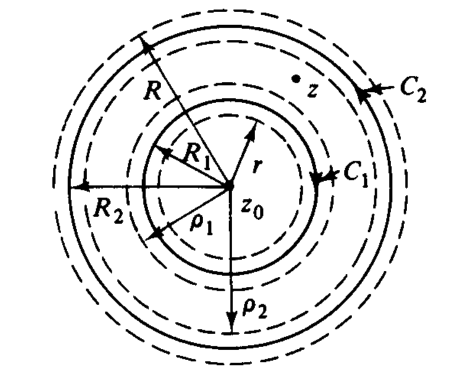
\includegraphics[width=0.4\textwidth]{figures/Laurent-proof-1.png}
		\caption{}
	\end{figure}

	The integral around $C_2$ can be treated the same way as in the proof of Taylor's Theorem. Now we treat the integral around $C_1$ in a symmetrical manner: 
	\begin{align*}
		\frac{1}{\zeta - z}&= \frac{1}{(\zeta - z_0) - (z - z_0)} \\
		&= \frac{1}{z-z_0} \frac{1}{\frac{\zeta - z_0}{z - z_0} - 1} \\
		&= -\frac{1}{z-z_0} \frac{1}{1 - a} & \text{where }a = \frac{\zeta - z_0}{z - z_0} \text{ and }|a|<1\\
		&= -\frac{1}{z-z_0} \left(1 + a^2 + \ldots + a^n + \frac{a^{n+1}}{1-a}\right) 	
	.\end{align*}

	Rewrite the integral:
	\begin{align*}
		&\frac{1}{2 \pi i}\int _{C_1} f(\zeta) \frac{-1}{z - z_0}\sum_{k = 0}^n a^k d\zeta\\
		&=\sum_{k=0}^{n}-\frac{1}{2 \pi i} \int _{C_1} f(\zeta) \frac{1}{z - z_0}a^k d\zeta\\
		&=\sum_{k=0}^{n}-\frac{1}{2 \pi i} (z-z_0)^{-k-1} \int _{C_1} f(\zeta) (\zeta - z_0)^k d\zeta\\
		&=\sum_{k=1}^{n+1}-\frac{1}{2 \pi i} (z-z_0)^{-k} \int _{C_1} f(\zeta) (\zeta - z_0)^{k-1} d\zeta\\
		&=\sum_{k=1}^{n+1}\left( -\frac{1}{2 \pi i} \int _{C_1} \frac{f(\zeta)}{(\zeta - z_0)^{-k+1}} d\zeta \right)  (z-z_0)^{-k} \\
		&=\sum_{k=1}^{n+1}\left( \frac{1}{2 \pi i} \int _{C} \frac{f(\zeta)}{(\zeta - z_0)^{-k+1}} d\zeta \right)  (z-z_0)^{-k}
	.\end{align*} 
	where $C$ is any positively oriented simple closed contour within the annulus with $z_0$ as its interior. We have a flip of sign due to flip of orientation. Now we have a convergent Laurent series exactly as desired in the theorem. It remains to show that the remainder term uniformly vanishes.

	The remainder term is
	\[
		T_n = \frac{1}{2 \pi i} \int_{C_1}- \frac{f(\zeta)}{z - z_0} \frac{a^{n+1}}{1-a}d \zeta 
		= \frac{1}{2 \pi i}\int_{C_1}\frac{f(\zeta) }{\zeta - z}\frac{(\zeta - z_0)^{n+1}}{(z- z_0)^{n+1}} d \zeta
	.\] 
	Apply main estimation. We have
	\begin{gather}
		|\zeta - z| \ge \rho_1 - R_1 \\
		| \zeta - z_0| = R_1 \\
		|z - z_0| \ge \rho_1
	\end{gather}
	Thus
	\begin{align*}
		|T_n| \le \frac{1}{2 \pi} (2 \pi R_1) \max_{\zeta \in C_1}f(\zeta) \frac{1}{\rho_1 - R_1} \left( \frac{R_1}{\rho_1} \right) ^{n+1}
	.\end{align*}
	The bound does not depend on $z$ and can be made arbitrarily small for large $n$, since $\frac{R_1}{\rho_1}<1$. Hence the convergence is uniform.
\end{proof}

Now we verify that any convergent ``Laurent-style series'' is the Laurent series of some function analytic in its annulus of convergence:
\begin{theorem}
	Let $\sum_{j=0}^{\infty} c_j\left(z-z_0\right)^j$ and $\sum_{j=1}^{\infty} c_{-j}\left(z-z_0\right)^{-j}$ be any two series with the following properties:\\
(i) $\sum_{j=0}^{\infty} c_j\left(z-z_0\right)^j$ converges for $\left|z-z_0\right|<R$,\\
(ii) $\sum_{j=1}^{\infty} c_{-j}\left(z-z_0\right)^{-j}$ converges for $\left|z-z_0\right|>r$, and\\
(iii) $r<R$.\\
Then there is a function $f(z)$, analytic for $r<\left|z-z_0\right|<R$, whose Laurent series in this annulus is given by $\sum_{j=-\infty}^{\infty} c_j\left(z-z_0\right)^j$.
\end{theorem}
\begin{proof}
	TBD.
\end{proof}

\subsection{Zeros}

\begin{definition}[Zero]
	A point $z_0$ is called a \textit{zero} of order $m$ for the function $f$ if $f$ is analytic at $z_0$ and $f$ and its first $m-1$ derivatives vanish at $z_0$, but $f^{(m)}\left(z_0\right) \neq 0$.

	In other words, the Laurent expansion at $z_0$ has no singular part, and $z^m$ is the first noznero term.
\end{definition}

\begin{theorem}[Canonical Representation]
Let $f$ be analytic at $z_0$. Then $f$ has a zero of order $m$ at $z_0$ if and only if $f$ can be written as
\[
f(z)=\left(z-z_0\right)^m g(z),
\]
where $g$ is analytic at $z_0$ and $g\left(z_0\right) \neq 0$.	
\end{theorem}
\begin{proof}
	It is assumed that
	\[
		f(z_0) = f^{(1)}(z_0) = \ldots = f^{(m-1)}(z_0) = 0 \neq  f^{(m)}(z_0)
	.\] 
	Hence its Taylor series around $z_0$ must be of the form
	\[
		a_m (z-z_0)^m + a_{m+1}(z-z_0)^{m+1} + \ldots
	.\] 
	which can be written as
	\[
		(z-z_0)^m \left( a_m + a_{m+1}(z-z_0) + \ldots \right) 
	.\] 
	Define $g(z) =  a_m + a_{m+1}(z-z_0) + \ldots $. We know that $g(z_0) = a_m \neq 0$ and $g$ analytic. 
\end{proof}


\begin{corollary}
	Zero of nonconstant analytic functions are isolated. If $f$ is an analytic function such that $f(z_0) = 0$, then either $f$ is identically in a neighborhood of $z_0$, or there is a punctured disk about $z_0$ in which $f$ has no zeros.
\end{corollary}
\begin{proof}
	Consider Taylor expansion of $f$ about $z_0$, and assume $f$ is not idencally zero. Then there is some finite $m$ such that $f$ has a zero of order $m$. Apply canonical representation, now $g$ is nonzero and continuous at $z_0$. So there exists a neighborhood such that $g$ is nonzero. Then $f$ is nonzero on some punctured disk within this neighborhood.
\end{proof}


\subsection{Isolated Singularities}

From Laurent's Theorem, around any isolated singularity $z_0$ of $f$ we have a Laurent Series about $z_0$ that converge to $f$ within a punctured disk about $z_0$.

\begin{definition}(Classification of Isolated Singularities)
	\begin{itemize}
		\item 
	If the Laurent series of $f$ at an isolated singularity $z_0$ has no singular part, we say $z_0$ is a \logseq{removable singularity} of $f$.
	\item
	If the Laurent series of $f$ at an isolated singularity $z_0$ has finitely many singular terms, we say $z_0$ is a \logseq{pole} of $f$ of order $m$, where $m$ is the greatest exponent of its nonzero singular term.
	\item
	If the Laurent series of $f$ at an isolated singularity $z_0$ has infinitely many singular terms, we say $z_0$ is an \logseq{essential singularity} of $f$.
	\end{itemize}
\end{definition}

\begin{theorem}(Equivalent Conditions for Removable Singularity)
	If $f$ has an isolated singularity at $z_0$, then the following statements are equivalent:
	\begin{enumerate}
		\item $z_0$ is a \logseq{removable singularity}.
		\item $|f|$ is bounded near $z_0$.
		\item $\lim_{z \to z_0} f$ exists.
		\item $f$ may be re-defined at $z_0$ so that $f$ is analytic at $z_0$.
	\end{enumerate}
\end{theorem}
\begin{proof}
	1,3,4 are equivalent by looking at Laurent (Taylor) expansion. Also 3 implies 2. Now we prove $2 \implies 1$.

	By Laurent's theorem, $f$ has Laurent expansion at $z_0$ and the coefficients are given by
	\[
		a_j = \frac{1}{2 \pi i} \oint_C f(\zeta) (\zeta - z_0)^{-j-1} d \zeta
	.\] 
	Let $C$ be a positively oriented circle with radius $\varepsilon>0$. We may assume $|f|\le M$ is bounded on some neighborhood containing the circle. Now
	\[
		|a_j| \le \frac{1}{2 \pi} (2 \pi \varepsilon) M \varepsilon^{-j-1}
	.\] 
	As $j\le -1$, we have $|a_j| \to 0$ as $\varepsilon \to 0$. Hence the singularity is removable.
\end{proof}

\begin{lemma}
	If $f$ has a pole of order $m$ at $z_0$, then $(z-z_0)^m f(z)$ has a removable singularity at $z_0$, and the limit is nonzero; also, $(a-a_0)^l f(z) \to  \infty $ as $z \to z_0$ whenever $0 \le  l < m$.
\end{lemma}
\begin{proof}
	Look at the Laurent expansion of $f$. It has the form
	\[
		f(z) = a_{-m}(z-z_0)^{-m} + \ldots + a_{-1}(z-z_0)^{-1} + a_0 + a_1 (z-z_0) + \ldots
	\] 
	where $a_{-m}\neq 0$.
	Hence
\[
	(z-z_0)^m f(z) = a_{-m} + \ldots + a_{-1}(z-z_0)^{m-1} + a_0(z-z_0)^m + a_1 (z-z_0)^{m+1} + \ldots
	.\]
	There is no negative power, the singularity at $z_0$ is removable. $a_{-m}\neq 0$ implies the limit is nonzero. Also, for any $l < m$,
	\[
		\left| (z-z_0)^l f(z) \right| =  \left| \frac{1}{(z-z_0)^{m - l}} (z-z_0)^m f(z) \right| \to  \infty 
	.\] 
	Since $(z-z_0)^m f(z) \to a_{-m}$ and $(z-z_0)^{-(m-l)} \to \infty $.
\end{proof}

\begin{theorem}(Equivalent Conditions for Pole Singularity)
	If $f$ has an isolated singularity at $z_0$, then the following statements are equivalent:
	\begin{enumerate}
		\item $z_0$ is a \logseq{pole}.
		\item $|f(z)| \to  \infty $ as $z \to  z_0$.
		\item $f(z) = (z-z_0)^{-m} g(z)$ for some integer $m>0$ and some $g$ analytic and nonzero at $z_0$.
	\end{enumerate}
\end{theorem}
\begin{proof}
	We proved $1 \implies 3$ and $3 \implies 2$ using the argument in the last lemma. It remains to prove $2 \implies 1$.

	If $|f(z)| \to \infty $ as $z \to  z_0$, then $|\frac{1}{f(z)}| \to  0$. Thus $z_0$ is a removable singularity of $\frac{1}{f}$. After removing the singularity, $\frac{1}{f}$ has a zero at $z_0$ of some order $m$. Hence by the lemma below, $f$ has a pole at $z_0$ of order $m$.
\end{proof}
\begin{lemma}(Zeros and Poles)
	We have the following implications:
	\begin{itemize}
		\item $f$ has a zero of order $m$ at $z_0$ $\implies$ $\frac{1}{f}$ has a pole of order $m$ at $z_0$.
		\item $f$ has a pole of order $m$ at $z_0$ $\implies$ $\frac{1}{f}$ has a removable singularity at $z_0$, and if we define $\frac{1}{f}(z_0) = 0$, then $\frac{1}{f}$ has a zero of order $m$ at $z_0$.
	\end{itemize}
\end{lemma}
\begin{proof}
	From canonical representation, $f(z) = (z-z_0)^m g(z)$ where $g(z_0)\neq 0$ and $g$ analytic at $z_0$ (and within domain of analyticity of  $f$ ). Hence $g(z)\neq 0$ within some neighbor of $z_0$. Hence $\frac{1}{g}$ analytic and nonzero within some neighborhood of $z_0$. Now simply take reciprocal.

	From the previous lemma, we can define  $g(z) = (z-z_0)^m f(z)$. Now $g$ has a removable singularity at $z_0$ and the limit $\lim_{z \to z_0} g(z)$ exists and is nonzero; so $\frac{1}{g}$ is analytic and nonzero in a neighborhood of $z_0$. Hence $\frac{1}{f}(z) = \frac{1}{g}(z) (z-z_0)^m$. Therefore, $\lim_{z \to z_0} \frac{1}{f}(z) = \lim_{z \to z_0} \frac{1}{g}(z) \lim_{z \to z_0} (z-z_0)^m = 0$. So by property of removable singularity we have desired result.
\end{proof}


\begin{theorem}[Casorati-Weierstrass Theorem]
	If  $f(z)$ has an essential singularity at $z_0$, then for any $w \in \mathbb{C}$ there exists a sequence $z_n \to  z_0$ such that $f(z_n) \to  w$. In other words, in any punctured neighborhood of  $z_0$, $f$ comes arbitrarily close to any complex number.
\end{theorem}
\begin{proof}
	Suppose $f$ is bounded away from $w \in \mathbb{C}$. Then in some punctured neighborhood $A$ of $z_0$, $\left| f(z) - w \right| \ge \delta>0$. Hence $\frac{1}{f(z) - w}$ is bounded in $A$. Therefore $\frac{1}{f(z) - w}$ has a removable singularity at $z_0$. Remove the singularity and call it $g$. Now $f = \frac{1}{g} + w$ and $g$ is analytic, so either $f$ is analytic at $z_0$ or $f$ has a pole at $z_0$. This is a contradiction because we assumed that $z_0$ is essential.
\end{proof}

There is a stronger version of the theorem, but the proof is beyond this course.
\begin{theorem}[Picard's Great Theorem]
	In every neighborhood of an essential singularity, $f$ takes every value in $\mathbb{C} $ with at most one exception.
\end{theorem}


\begin{theorem}(Equivalent Conditions for Essential Singularity)
	If $f$ has an isolated singularity at $z_0$, then the following statements are equivalent:
	\begin{enumerate}
		\item $z_0$ is an \logseq{essential singularity}.
		\item $|f|$ is unbounded near $z_0$ but does not converge to $\infty $ as $z \to  z_0$.
		\item Within every neighborhood of $z_0$, $f(z) = w$ has solution for any $w \in \overline{\mathbb{C}} $, except possibly $\le 2$ values in $\overline{\mathbb{C}} $.
	\end{enumerate}
\end{theorem}
\begin{proof}
	$1 \iff  2$ follows from property of removable and pole singularity. $3$ is stated without proving.
\end{proof}


\subsubsection{Identity Theorem}
\begin{lemma}
	Let $f$ be analytic in $D$, and define $E = \{z \in D: f(z) = 0\} $. Let $L$ be the set of accumulation points of $E$. Then $L$ is clopen in $D$.
\end{lemma}
\begin{proof}
	By property of accumulation point, $L$ is closed. We now prove it is open. Let $z_0 \in L$ and consider taylor expansion $f(z) = \sum_{n=0}^{\infty} a_n (z-z_0)^n$ that converges in $B(z_0, r)$ for some $r>0$. If the expansion is identically zero then we are done; otherwise $f$ has a zero of order $m$ for some finite $m>0$. Then $f(z) = (z-z_0)^m g(z)$ where $g(z)$ is analytic and nonzero at $z_0$. Hence $g(z)$ is nonzero in a neighborhood of $z_0$. Hence $f(z)$ is nonzero in a neighborhood of $z_0$. But then $z_0$ is an isolated point, a contradiction. Hence indeed we have  $B(z_0, r) \subset L$, hence $L$ open.
\end{proof}

\begin{theorem}[Identity Theorem]
	Let $f, g$ be analytic on a domain $D \subset \mathbb{C}$. If $E \subset D$ has some non-isolated points and $f = g$ on $E$, then $f = g$ on $D$.
\end{theorem}
\begin{proof}
	Apply the lemma to $f-g$, so they are equal on a clopen subset. But since $D$ is connected, the only clopen subset of it are $\emptyset $ and $D$ itself, so $f-g \equiv 0$ on $D$.
\end{proof}

\begin{example}
	As a special case, if $f(z) = 0$ on a set with accumulation point, then $f(z) = 0$ everywhere.
\end{example}
\begin{example}
	Using this theorem, we can extend identities from real axis to the complex plane. For example, consider $f(z) = \cos^2 z + \sin^2 z$ and $g(z) = 1$, and we know $\cos^2 z + \sin^2 z = 1$ on $\mathbb{R}$. Hence the same holds on $\mathbb{C}$.
\end{example}

\subsection{Point at Infinity}

We extend the definition of singularities to the point $\infty $ in $\overline{\mathbb{C}} $.

\begin{definition}

	We say $f(z)$ has a type of singularity at $\infty $, if $f(\frac{1}{z})$ has the type of singularity at $0$. Specifically,
	\begin{itemize}
		\item 
	We say $f(z)$ is analytic at $\infty $ if $f(\frac{1}{z})$ is analytic (or has removable singularity) at $w = 0$.
\item
	We say $f(z)$ has a pole of order $m$ at $\infty $ if $f(\frac{1}{w})$ has a pole of order $m$ at $0$.
\item 
	We say $f(z)$ has an essential singularity at $\infty $ if $f(\frac{1}{w})$ has an essential singularity at $0$.
	\end{itemize}
\end{definition}
\begin{proposition}
	(Criterions for singularity at infinity)
	The following hold:
	\begin{enumerate}
		\item $f(z)$ is analytic at $\infty $ if $|f(z)|$ is bounded for large $|z|$.
		\item $f(z)$ has a pole at $\infty $ if $f(z) \to \infty $ as  $z\to \infty $.
		\item $f(z)$ has essential singularity if $f(z)$ is unbounded and diverge as $z \to \infty $.
	\end{enumerate}
\end{proposition}

\begin{example}
Find all the functions $f$ that are analytic everywhere in the extended complex plane.

Solution. Since $f$ is analytic at $\infty$, it is bounded for, say, $|z|>M$. By continuity, $f$ is also bounded for $|z| \leq M$. Consequently, $f$ is a bounded entire function. Hence $f$ is constant, by Liouville's theorem.
\end{example}
\begin{example}
Classify all the functions that are everywhere analytic in the extended complex plane except for a pole at one point.

Solution. If $f(z)$ has a pole, say, of order $m$ at some finite point $z_0$, then the Laurent series for $f$
\[
f(z)=\frac{a_{-m}}{\left(z-z_0\right)^m}+\frac{a_{-m+1}}{\left(z-z_0\right)^{m-1}}+\cdots+\frac{a_{-1}}{z-z_0}+\sum_{n=0}^{\infty} a_n\left(z-z_0\right)^n
\]
converges for all $z \neq z_0$. Moreover, since we are assuming that $z_0 \neq \infty$, the function $f$ must be analytic, and hence bounded, at $\infty$. From Eq. (2), then, we see that the entire function defined by the series $\sum_{n=0}^{\infty} a_n\left(z-z_0\right)^n$ is also bounded at $\infty$; thus it must be constant, that is, equal to $a_0$. Therefore, the most general form for such a function $f$ is
\[
f(z)=\frac{a_{-m}}{\left(z-z_0\right)^m}+\frac{a_{-m+1}}{\left(z-z_0\right)^{m-1}}+\cdots+\frac{a_{-1}}{z-z_0}+a_0 .
\]
If the pole occurs at $z=\infty$, then $f(1 / w)$ has a pole at the origin and can be expressed in the form
\[
f\left(\frac{1}{w}\right)=\frac{a_{-m}}{w^m}+\frac{a_{-m+1}}{w^{m-1}}+\cdots+\frac{a_{-1}}{w}+\sum_{n=0}^{\infty} a_n w^n .
\]
Since $f(z)$ is bounded near $z=0$, it follows that $f(1 / w)$ is bounded for large $|w|$, and, as before, we conclude that $a_n=0$ for $n>0$. Hence Eq. (4) becomes
\[
f(z)=a_{-m} z^m+a_{-m+1} z^{m-1}+\cdots+a_{-1} z+a_0 ;
\]
that is, $f(z)$ is a polynomial in $z$.
\end{example}


